\subsection{Serie 6}%
\label{sub:serie_6}

\paragraph{Aufgabe 1}%
\label{par:aufgabe_1}

Erklären Sie: in einem Spiel in strategischer Form kann ein Spieler $i$ nicht
mehr als eine schwach (bzw. strikt) dominante Strategie haben.

\paragraph{Aufgabe 2}%
\label{par:aufgabe_2}

Betrachten Sie folgendes Spiel in extensiver Form:
\begin{center}
  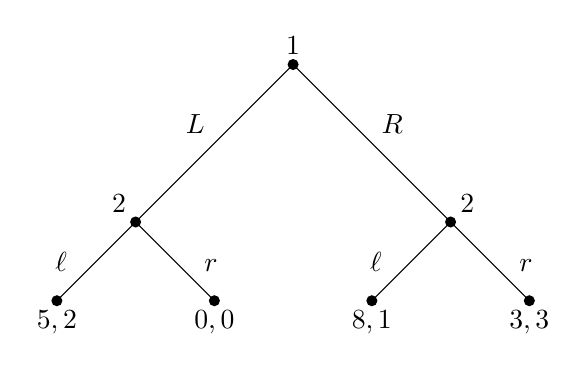
\begin{tikzpicture}
    \fill (0,0) circle (2pt) node [above] {$1$};
    \fill (-2,-2) circle (2pt) node [above left] {$2$};
    \fill (2,-2) circle (2pt) node [above right] {$2$};
    \fill (-3,-3) circle (2pt) node [below] {$5,2$};
    \fill (-1,-3) circle (2pt) node [below] {$0,0$};
    \fill (1,-3) circle (2pt) node [below] {$8,1$};
    \fill (3,-3) circle (2pt) node [below] {$3,3$};

    \draw (0,0) -- (-2,-2) node [midway,above left] {$L$};
    \draw (-2,-2) -- (-3,-3) node [near end,above left] {$\ell$};
    \draw (-2,-2) -- (-1,-3) node [near end,above right] {$r$};
    \draw (0,0) -- (2,-2) node [midway,above right] {$R$};
    \draw (2,-2) -- (1,-3) node [near end,above left] {$\ell$};
    \draw (2,-2) -- (3,-3) node [near end,above right] {$r$};
  \end{tikzpicture}
\end{center}

\begin{enumerate}
  \item Beschreiben Sie in Worten die Spielabfolge, potentielle Aktionen der Agenten und
    deren Informationen auf jeder Stufe.

  \item Erklären Sie den Unterschied zwischen einer Aktion und einer Strategie. Geben Sie
    für jeden Spieler ein Beispiel einer Aktion und ein Beispiel einer Strategie.

  \item Definieren Sie das Lösungskonzept Nash-GG (NGG). Was sind die reinen NGG dieses
    Spiels? Was sind die Ergebnisse dieser NGG?

  \item Definieren Sie ein Teilspiel und ein teilspielperfektes Nash-GG (SPNE) informell.
    Was sind die reinen SPNE dieses Spiels? Was sind die Ergebnisse dieser SPNE?

  \item Finden Sie das Konzept eines SPNE attraktiv? Ist es im Kontext dieses Spiels
    angemessen?
\end{enumerate}

\paragraph{Aufgabe 3}%
\label{par:aufgabe_3}

Betrachten Sie folgendes Spiel in extensiver Form:
\begin{center}
  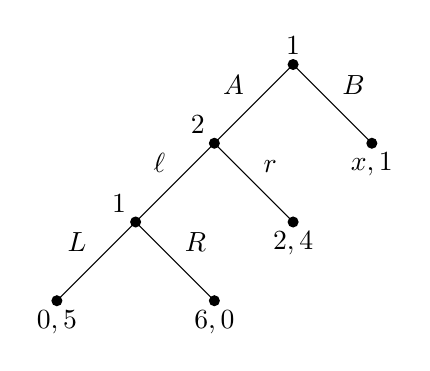
\begin{tikzpicture}
    \fill (0,0) circle (2pt) node [below] {$0,5$};
    \fill (2,0) circle (2pt) node [below] {$6,0$};
    \fill (1,1) circle (2pt) node [above left] {$1$};
    \fill (3,1) circle (2pt) node [below] {$2,4$};
    \fill (2,2) circle (2pt) node [above left] {$2$};
    \fill (4,2) circle (2pt) node [below] {$x,1$};
    \fill (3,3) circle (2pt) node [above] {$1$};

    \draw (3,3) -- (2,2) node [midway, above left] {$A$};
    \draw (3,3) -- (4,2) node [midway, above right] {$B$};
    \draw (2,2) -- (1,1) node [midway, above left] {$\ell$};
    \draw (2,2) -- (3,1) node [midway, above right] {$r$};
    \draw (1,1) -- (0,0) node [midway, above left] {$L$};
    \draw (1,1) -- (2,0) node [midway, above right] {$R$};
  \end{tikzpicture}
\end{center}

\begin{enumerate}
  \item Besttimmen Sie die Strategien der Spieler.
  \item Finden Sie die Menge der NGG dieses Spiels.
  \item Finden Sie die Menge der SPNE dieses Spieles für $x = 7,4,1$.
  \item Finden Sie das Konzept eines SPNE attraktiv?
    Vergleichen Sie die Situation für $x=7,4,1$.
\end{enumerate}

\paragraph{Aufgabe 4}%
\label{par:aufgabe_4}

Betrachten Sie folgendes Spiel in extensiver Form:
\begin{center}
  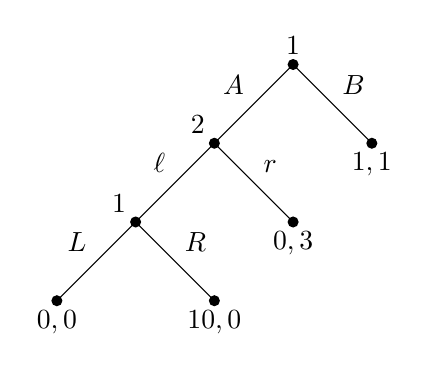
\begin{tikzpicture}
    \fill (0,0) circle (2pt) node [below] {$0,0$};
    \fill (2,0) circle (2pt) node [below] {$10,0$};
    \fill (1,1) circle (2pt) node [above left] {$1$};
    \fill (3,1) circle (2pt) node [below] {$0,3$};
    \fill (2,2) circle (2pt) node [above left] {$2$};
    \fill (4,2) circle (2pt) node [below] {$1,1$};
    \fill (3,3) circle (2pt) node [above] {$1$};

    \draw (3,3) -- (2,2) node [midway, above left] {$A$};
    \draw (3,3) -- (4,2) node [midway, above right] {$B$};
    \draw (2,2) -- (1,1) node [midway, above left] {$\ell$};
    \draw (2,2) -- (3,1) node [midway, above right] {$r$};
    \draw (1,1) -- (0,0) node [midway, above left] {$L$};
    \draw (1,1) -- (2,0) node [midway, above right] {$R$};
  \end{tikzpicture}
\end{center}

\begin{enumerate}
  \item Finden Sie die Menge NGG dieses Spiels.
  \item Finden Sie die Menge der SPNE dieses Spieles.
  \item Nehmen Sie nun an, dass Spieler 2 mit Wahrscheinlichkeit $\beta \in (0,1)$
    irrational ist und mit der selben Wahrscheinlichkeit $\ell, r$ wählt.
    Wie groß muss $\beta$ sein, damit es für Spieler $1$ optimal ist $A$ zu wählen?
\end{enumerate}

\paragraph{Aufgabe 5}%
\label{par:aufgabe_5}

In einer Amerikanischen Fernsehshow wird den Spielern die Wahl zwischen dem Öffnen einer
von drei Türen (rot, grün, blau) angeboten.
Hinter einer Tür verbirgt sich ein Preis, hinter den anderen nichts.
Die Spieler haben keinen Grund anzunehmen, dass eine der Türen mit höherer
Wahrscheinlichkeit zu einem Preis führt als eine andere.
Der Quizmaster weiß, hinter welcher Tür der Preis liegt.
Nachdem ein Spieler eine der Türen gewählt (aber noch nicht geöffnet) hat, \emph{muss} der
Quizmaster eine der anderen Türen öffnen.
Der Spieler kann sich dann entscheiden, ob er bei der von ihm ursprünglich gewählten Tür
bleibt, oder ob er zu einer anderen Tür wechselt.
Nehmen Sie an, dass die Spieler die Wahrscheinlichkeit den Preis zu bekommen maximieren,
während der Quizmaster diese Wahrscheinlichkeit minimieren möchte.

\begin{enumerate}
  \item Beschreiben Sie eine optimale Strategie des Quizmasters.
    Nehmen Sie im Weiteren an, dass der Quizmaster diese Strategie verfolgt.

  \item Was sollte der Spieler tun, wenn er gefragt wird, ob er wechseln möchte?
    Begründen Sie Ihre Antwort.
\end{enumerate}
